Unter Verwendung des Virialsatzes berechnete der Schweizer Physiker Fritz Zwickey im Jahr 1933 anhand von Messungen der Dichteverteilung die mittlere Geschwindigkeit von Materie im Coma Cluster.
Die Berechnungen ergaben, dass die Masse um ein 400 faches kleiner ist, als zuvor über die Rotverschiebung vorhergesagt.
Selbst unter der Annahme, dass sich das Comasystem in einem nicht stationären Zustand befindet, verringert sich sein Ergebnis nur um einen Faktor ein Halb.
Um diese erhebliche Diskrepanz zu erklären gibt es verschiedene Ansätze.
Das Comasystem könnte beispielsweise mit der Zeit auseinanderfliegen.
Am Ende dieser Expansion gäbe es Einzelnebel mit Eigengeschwindigkeiten von $\SI{1000}{\kilo\meter.\second^{-1}}$ bis $\SI{2000}{\kilo\meter.\second^{-1}}$.
Da Einzelnebel mit solchen Geschwindigkeiten nicht beobachtet wurden, postulierte Fritz Zwickey weitere nicht leuchtende Materie.
Er nannte diese Dunkle Materie.\cite{zwicky}

Anfänglich fand die Vorstellung von Dunkler Materie nicht viele Anhänger.
Erst 50 Jahre später als Vera Rubin die Rotationskurven 21 verschiedener spiraler Galaxien untersuchte, erwachte weiterführendes wissenschaftliches Interesse.
Im Rahmen der Arbeit wurde festgestellt, dass die beobachtete Geschwindigkeitsverteilung sich von der berechneten Geschwindigkeitsverteilung erheblich unterscheidet.
Aus dem Kepplerschen Gesetz folgt, dass die Geschwindigkeitsverteilung $v(R)$ bei bekannter Massenverteilung $M(R)$ durch
\begin{equation}
v(R) = \sqrt{\frac{GM(R)}{R}}
\label{eq:Keppler}
\end{equation}
gegeben ist.
Anhand der Leuchtkraft von Galaxien lässt sich die Verteilung leuchtender Materie messen.
Bei Spiralgalaxien ist die Dichte in der Nähe des Zentrums am größten.
Nach außen hin bildet sich eine rotierende Scheibe (\textit{disk}) von Sternen und Gasen geringerer Dichte.
In der Summe nimmt die Masse bei kleinen Abständen schnell zu.
Bei großen Abständen allerdings nur noch proportional zu $\exp(-R)$.
Daher sollte die Rotationsgeschwindigkeit bei großen Abständen eine $1/\sqrt{R}$ Abhängigkeit aufweisen.

Entgegen allen Erwartungen fand Vera Rubin, dass die Geschwindigkeit bei großen Entfernungen nicht abnimmt, sondern weiter ansteigt oder konstant bleibt.
Abbildung \ref{fig:ROT_NGC3198} zeigt eine gemessene Rotationskurve der Galaxie NGC 3198.
Zu sehen ist, dass bei großen Entfernungen die \textit{disk} aus leuchtender Materie nicht ausreicht um die hohe Geschwindigkeit zu erklären.
Zusätzlich ist eine \textit{halo}-artige Verteilung von Dunkler Materie nötig, damit das gewünschte Verhalten erreicht wird.
Die Massenverteilung der Dunklen Materie kann aus der Diskrepanz zwischen gemessener und erwarteter Masse berechnet werden, indem das Kepplersche Gesetz \eqref{eq:Keppler} ausgenutzt wird.
\begin{align}
v(R)_{\mathrm{DM}}^2 &= v_{\Sigma}(R)^2 - v(R)_{\mathrm{lum}}^2 \\
\stackrel{\eqref{eq:Keppler}}{\Rightarrow} M(R)_{\mathrm{DM}} &= \frac{R}{G}\left(v_{\Sigma}(R)^2 - v(R)_{\mathrm{lum}}^2\right)
\end{align}
Die gesamte Masse bleibt allerdings unbestimmt, da die Ausdehnung des Dunkle Materie \textit{halos} unbekannt ist.\cite{VRubin}

\begin{figure}[!t]
\begin{center}
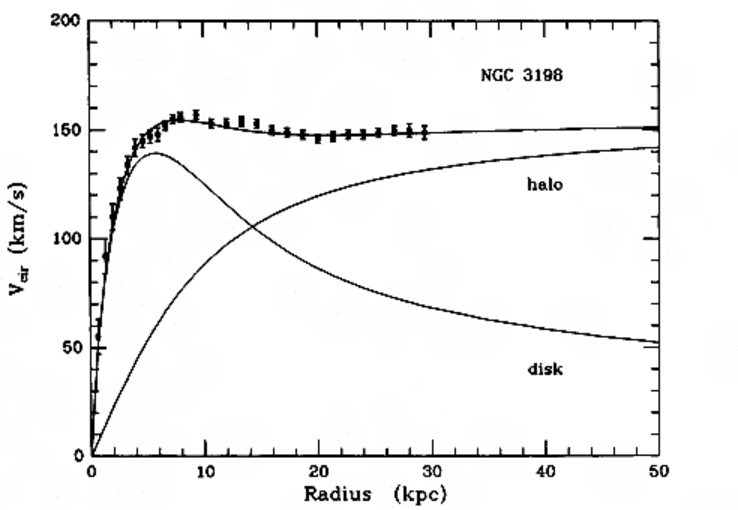
\includegraphics[width=0.8\textwidth]{./fig/NGC3198.pdf}
\end{center}
\caption{Roatationskurve der spiralen Galaxie NGC 3198.
Aufgrund der erwartete Massenverteilung berechnete Geschwindigkeitsverteilung(\textit{disk}).
Gemessene Geschwindigkeitsverteilung(NGC 3198).
Benötigte Dunkle Materie Geschwindigkeitsverteilung um die Beobachtungen zu erklären(\textit{halo}).\cite{NGC}}
\label{fig:ROT_NGC3198}
\end{figure}

Weitere Evidenz für die Existenz von Dunkler Materie lässt sich aus Beobachtungen von kollidierenden Clustern gewinnen.
Bei der Kollision beeinflussen sich die stellaren Bestandteile nicht und fliegen deshalb unverändert weiter.
Das interstellare Plasma, welches den Großteil der leuchtenden Materie ausmacht, wird vor allem aufgrund von elektromagnetischer Wechselwirkung abgebremst und entkoppelt deshalb von dem ursprünglichen Cluster.
Durch die Wechselwirkung fängt das Plasma an zu leuchten.
Primär durch Aussenden von Bremsstrahlung im Röntgenbereich.

Das Rechte Bild in Abbildung \ref{fig:BulletC} zeigt eine Aufnahme des Bullet Clusters vom Chandra Teleskop im Röntgenspektrum.
Stellen größter Intensität sind rot bis weiß gefärbt. 
Zusätzlich kann durch den schwachen Gravitationslinseneffekt das Gravitationspotential bestimmt werden.
Äquipotentiallinien sind in \ref{fig:BulletC} grün dargestellt.
Die Messung zeigt, dass der Schwerpunkt nicht wie angenommen im Zentrum der leuchtenden Materie liegt, sondern unbeeinflusst weiter fliegt.
Diese Beobachtungen könnten durch nicht leuchtende, nicht wechselwirkende Dunkle Materie erklärt werden.\cite{BulletC}


\begin{figure}[!b]
\begin{center}
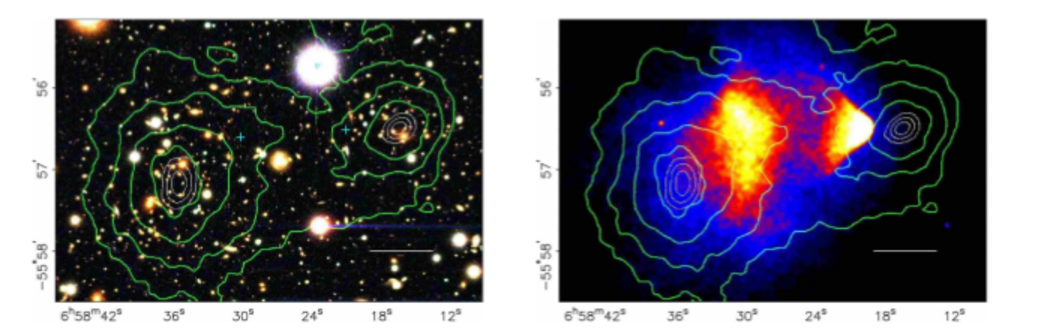
\includegraphics[width=\textwidth]{./fig/Bullet.pdf}
\end{center}
\caption{Links:Bild des Bullet Cluster. 
Aufnahme des Magellan Teleskop.
Rechts: Röntgenaufnahme des Bullet Cluster vom Chandra Teleskop.
Die Konturen zeigen die durch den schwachen Gravitationslinseneffekt erwartete Massenverteilung.\cite{BulletC}}
\label{fig:BulletC}
\end{figure}



